% !TEX root = ../main.tex

\section{Results and discussion}

Feedstock characterization, batch reactor, and CSTR model results are discussed in this section.

\subsection{Feedstock characterization}

Table \ref{tab:basis} presents the proximate and ultimate analysis data on an as-determined (AD), as-received (AR), dry (D), dry ash-free (DAF), and CHO basis. The reported H and O for the ultimate analysis data does not include the H and O in the moisture; therefore, the total value for the as-determined basis (AD column) excludes the moisture percentage.

\newpage
\begin{longtable}{lrrrrr}
    \caption{Proximate and ultimate analysis basis values for each feedstock given as wt. \%. Reported H and O values for ultimate analysis AD basis excludes H and O in moisture.}
    \label{tab:basis} \\

    \textbf{Residues} & AD & AR & D & DAF & CHO \\
    \hline \\
    FC       & 20.72  & 17.33  & 21.79  & 22.13  & -- \\
    VM       & 72.92  & 60.99  & 76.69  & 77.88  & -- \\
    ash      & 1.45   & 1.21   & 1.53   & --     & -- \\
    moisture & 4.92   & 20.58  & --     & --     & -- \\
    total    & 100.01 & 100.01 & 100.01 & 100.01 & -- \\
    \\
    C        & 49.63  & 38.71 & 52.20 & 53.01 & 53.31 \\
    H        & 6.52   & 4.66  & 6.28  & 6.38  & 6.41 \\
    O        & 41.87  & 29.25 & 39.44 & 40.05 & 40.28 \\
    N        & 0.49   & 0.38  & 0.52  & 0.52  & -- \\
    S        & 0.04   & 0.03  & 0.04  & 0.04  & -- \\
    ash      & 1.45   & 1.13  & 1.53  & --    & -- \\
    moisture & (4.92) & 25.84 & --    & --    & -- \\
    total    & 100    & 100   & 100   & 100   & 100 \\
    \\

    \textbf{Stem wood} & AD & AR & D & DAF & CHO \\
    \hline \\
    FC       & 16.79  & 13.10  & 17.41  & 17.46  & -- \\
    VM       & 79.40  & 61.93  & 82.32  & 82.56  & -- \\
    ash      & 0.28   & 0.22   & 0.29   & --     & -- \\
    moisture & 3.55   & 24.77  & --     & --     & -- \\
    total    & 100.02 & 100.02 & 100.02 & 100.02 & -- \\
    \\
    C        & 48.89  & 38.13  & 50.69  & 50.84  & 50.94 \\
    H        & 6.53   & 4.78   & 6.36   & 6.38   & 6.39 \\
    O        & 44.12  & 31.95  & 42.48  & 42.60  & 42.68 \\
    N        & 0.18   & 0.14   & 0.19   & 0.19   & -- \\
    S        & 0.01   & 0.01   & 0.01   & 0.01   & -- \\
    ash      & 0.28   & 0.22   & 0.29   & --     & -- \\
    moisture & (3.55) & 24.77  & --     & --     & -- \\
    total    & 100.01 & 100.01 & 100.01 & 100.01 & 100.01 \\
    \\

    \textbf{Bark} & AD & AR & D & DAF & CHO \\
    \hline \\
    FC       & 27.16  & 21.18  & 28.85  & 29.07  & -- \\
    VM       & 66.29  & 51.71  & 70.42  & 70.94  & -- \\
    ash      & 0.70   & 0.55   & 0.74   & --     & -- \\
    moisture & 5.86   & 26.57  & --     & --     & -- \\
    total    & 100.01 & 100.01 & 100.01 & 100.01 & -- \\
    \\
    C        & 51.84  & 40.44  & 55.07  & 55.48  & 55.69 \\
    H        & 6.14   & 4.28   & 5.83   & 5.87   & 5.89 \\
    O        & 40.97  & 27.90  & 37.99  & 38.28  & 38.42 \\
    N        & 0.34   & 0.27   & 0.36   & 0.36   & -- \\
    S        & 0.02   & 0.02   & 0.02   & 0.02   & -- \\
    ash      & 0.70   & 0.55   & 0.74   & --     & -- \\
    moisture & (5.86) & 26.57  & --     & --     & -- \\
    total    & 100.01 & 100.01 & 100.01 & 100.01 & 100.01 \\
    \\

    \textbf{Needles} & AD & AR & D & DAF & CHO \\
    \hline \\
    FC       & 23.26  & 18.14  & 24.08  & 25.06  & -- \\
    VM       & 69.54  & 54.24  & 72.00  & 74.94  & -- \\
    ash      & 3.78   & 2.95   & 3.91   & --     & -- \\
    moisture & 3.42   & 24.67  & --     & --     & -- \\
    total    & 100    & 100    & 100    & 100    & -- \\
    \\
    C        & 50.22  & 39.17  & 52.00  & 54.12  & 54.71 \\
    H        & 6.22   & 4.55   & 6.04   & 6.29   & 6.36 \\
    O        & 38.77  & 27.87  & 37.00  & 38.51  & 38.93 \\
    N        & 0.92   & 0.72   & 0.95   & 0.99   & -- \\
    S        & 0.09   & 0.07   & 0.09   & 0.10   & -- \\
    ash      & 3.78   & 2.95   & 3.91   & --     & -- \\
    moisture & (3.42) & 24.67  & --     & --     & -- \\
    total    & 100    & 100    & 100    & 100    & 100 \\
    \\

    \textbf{Bark + needles} & AD & AR & D & DAF & CHO \\
    \hline \\
    FC       & 24.35  & 18.99  & 25.59  & 26.29  & -- \\
    VM       & 68.30  & 53.27  & 71.78  & 73.73  & -- \\
    ash      & 2.52   & 1.97   & 2.65   & --     & -- \\
    moisture & 4.85   & 25.78  & --     & --     & -- \\
    total    & 100.02 & 100.02 & 100.02 & 10.02  & -- \\
    \\
    C        & 50.35  & 39.27  & 52.92  & 54.36  & 54.79 \\
    H        & 6.18   & 4.40   & 5.92   & 6.09   & 6.13 \\
    O        & 40.21  & 28.00  & 37.73  & 38.76  & 39.07 \\
    N        & 0.67   & 0.52   & 0.70   & 0.72   & -- \\
    S        & 0.06   & 0.05   & 0.06   & 0.06   & -- \\
    ash      & 2.52   & 1.97   & 2.65   & --     & -- \\
    moisture & (4.85) & 25.78  & --     & --     & -- \\
    total    & 99.99  & 99.99  & 99.99  & 99.99  & 99.99 \\
    \\

    \textbf{Residues (rep 1)} & AD & AR & D & DAF & CHO \\
    \hline \\
    FC       & 20.78  & 16.21  & 21.92  & 22.31  & -- \\
    VM       & 72.37  & 56.45  & 76.34  & 77.69  & -- \\
    ash      & 1.65   & 1.29   & 1.74   & --     & -- \\
    moisture & 5.20   & 26.06  & --     & --     & -- \\
    total    & 100    & 100    & 100    & 100    & -- \\
    \\
    C        & 49.82  & 38.86  & 52.55  & 53.48  & 53.85 \\
    H        & 6.56   & 4.66   & 6.31   & 6.42   & 6.46 \\
    O        & 41.34  & 28.64  & 38.74  & 39.42  & 39.69 \\
    N        & 0.58   & 0.45   & 0.61   & 0.62   & -- \\
    S        & 0.05   & 0.04   & 0.05   & 0.05   & -- \\
    ash      & 1.65   & 1.29   & 1.74   & --     & -- \\
    moisture & (5.20) & 26.06  & --     & --     & -- \\
    total    & 100    & 100    & 100    & 100    & 100 \\
    \\

    \textbf{Residues:bark:needles 1:1:1} & AD & AR & D & DAF & CHO \\
    \hline \\
    FC       & 23.75  & 18.52  & 25.05  & 25.60  & -- \\
    VM       & 69.02  & 53.84  & 72.80  & 74.41  & -- \\
    ash      & 2.05   & 1.60   & 2.16   & --     & -- \\
    moisture & 5.19   & 26.05  & --     & --     & -- \\
    total    & 100.01 & 100.01 & 100.01 & 100.01 & -- \\
    \\
    C        & 50.58  & 39.45  & 53.35  & 54.53  & 54.91 \\
    H        & 6.31   & 4.47   & 6.04   & 6.18   & 6.22 \\
    O        & 40.43  & 27.94  & 37.78  & 38.62  & 38.88 \\
    N        & 0.59   & 0.46   & 0.62   & 0.64   & -- \\
    S        & 0.05   & 0.04   & 0.05   & 0.05   & -- \\
    ash      & 2.05   & 1.60   & 2.16   & --     & -- \\
    moisture & (5.19) & 26.05  & --     & --     & -- \\
    total    & 100.01 & 100.01 & 100.01 & 100.01 & 100.01 \\
    \\

    \textbf{Residues:bark:needles 1:2:2} & AD & AR & D & DAF & CHO \\
    \hline \\
    FC       & 24.12  & 18.81  & 25.47  & 26.02  & -- \\
    VM       & 68.57  & 53.48  & 72.40  & 73.98  & -- \\
    ash      & 2.02   & 1.58   & 2.13   & --     & -- \\
    moisture & 5.29   & 26.13  & --     & --     & -- \\
    total    & 100    & 100    & 100    & 100    & -- \\
    \\
    C        & 50.86  & 39.67  & 53.70  & 54.87  & 55.25 \\
    H        & 6.24   & 4.41   & 5.96   & 6.09   & 6.14 \\
    O        & 40.24  & 27.72  & 37.53  & 38.34  & 38.61 \\
    N        & 0.58   & 0.45   & 0.61   & 0.63   & -- \\
    S        & 0.06   & 0.05   & 0.06   & 0.06   & -- \\
    ash      & 2.02   & 1.58   & 2.13   & --     & -- \\
    moisture & (5.29) & 26.13  & --     & --     & -- \\
    total    & 100    & 100    & 100    & 100    & 100 \\
    \\

    \textbf{Air classified 10 Hz} & AD & AR & D & DAF & CHO \\
    \hline \\
    FC       & 19.92  & 15.54  & 20.66  & 20.86  & -- \\
    VM       & 75.59  & 58.96  & 78.39  & 79.14  & -- \\
    ash      & 0.92   & 0.72   & 0.95   & --     & -- \\
    moisture & 3.57   & 24.78  & --     & --     & -- \\
    total    & 100    & 100    & 100    & 100    & -- \\
    \\
    C        & 50.16  & 39.12  & 52.02  & 52.52  & 52.74 \\
    H        & 6.46   & 4.73   & 6.28   & 6.35   & 6.37 \\
    O        & 42.06  & 30.33  & 40.33  & 40.72  & 40.89 \\
    N        & 0.37   & 0.29   & 0.38   & 0.39   & -- \\
    S        & 0.03   & 0.02   & 0.03   & 0.03   & -- \\
    ash      & 0.92   & 0.72   & 0.95   & --     & -- \\
    moisture & (3.57) & 24.78  & --     & --     & -- \\
    total    & 100    & 100    & 100    & 100    & 100 \\
    \\

    \textbf{Air classified 28 Hz} & AD & AR & D & DAF & CHO \\
    \hline \\
    FC       & 18.68  & 14.57  & 19.54  & 19.67  & -- \\
    VM       & 76.31  & 59.52  & 79.83  & 80.34  & -- \\
    ash      & 0.61   & 0.48   & 0.64   & --     & -- \\
    moisture & 4.41   & 25.44  & --     & --     & -- \\
    total    & 100.01 & 100.01 & 100.01 & 100.01 & -- \\
    \\
    C        & 48.93  & 38.17  & 51.19  & 51.52  & 51.67 \\
    H        & 6.42   & 4.62   & 6.20   & 6.24   & 6.26 \\
    O        & 43.77  & 31.09  & 41.69  & 41.96  & 42.08 \\
    N        & 0.26   & 0.20   & 0.27   & 0.27   & -- \\
    S        & 0.02   & 0.02   & 0.02   & 0.02   & -- \\
    ash      & 0.61   & 0.48   & 0.64   & --     & -- \\
    moisture & (4.41) & 25.44  & --     & --     & -- \\
    total    & 100.01 & 100.01 & 100.01 & 100.01 & 100.01 \\
    \\

    \textbf{Whole tree 13 yr} & AD & AR & D & DAF & CHO \\
    \hline \\
    FC       & 19.15  & 14.94  & 19.89  & 19.98  & -- \\
    VM       & 76.72  & 59.84  & 79.68  & 80.04  & -- \\
    ash      & 0.44   & 0.34   & 0.46   & --     & -- \\
    moisture & 3.71   & 24.89  & --     & --     & -- \\
    total    & 100.02 & 100.02 & 100.02 & 100.02 & -- \\
    \\
    C        & 49.32  & 38.47  & 51.22  & 51.46  & 51.63 \\
    H        & 6.44   & 4.70   & 6.26   & 6.29   & 6.31 \\
    O        & 43.48  & 31.34  & 41.73  & 41.93  & 42.07 \\
    N        & 0.30   & 0.23   & 0.31   & 0.31   & -- \\
    S        & 0.02   & 0.02   & 0.02   & 0.02   & -- \\
    ash      & 0.44   & 0.34   & 0.46   & --     & -- \\
    moisture & (3.71) & 24.89  & --     & --     & -- \\
    total    & 100    & 100    & 100    & 100    & 100 \\
    \\

    \textbf{Stem wood 13 yr} & AD & AR & D & DAF & CHO \\
    \hline \\
    FC       & 18.60  & 14.51  & 19.13  & 19.19  & -- \\
    VM       & 78.37  & 61.13  & 80.59  & 80.84  & -- \\
    ash      & 0.30   & 0.23   & 0.31   & --     & -- \\
    moisture & 2.75   & 24.14  & --     & --     & -- \\
    total    & 100.02 & 100.02 & 100.02 & 100.02 & -- \\
    \\
    C        & 49.40  & 38.53  & 50.80  & 50.95  & 51.07 \\
    H        & 6.41   & 4.76   & 6.27   & 6.29   & 6.31 \\
    O        & 43.68  & 32.17  & 42.40  & 42.54  & 42.63 \\
    N        & 0.21   & 0.16   & 0.22   & 0.22   & -- \\
    S        & 0.01   & 0.01   & 0.01   & 0.01   & -- \\
    ash      & 0.30   & 0.23   & 0.31   & --     & -- \\
    moisture & (2.75) & 24.14  & --     & --     & -- \\
    total    & 100.01 & 100.01 & 100.01 & 100.01 & 100.01 \\
\end{longtable}

Using the chemical analysis measurement data from Tables \ref{tab:chemical-1} and \ref{tab:chemical-2}, the dry ash-free basis (DAF) values are calculated using Equation \ref{eq:chem-daf}. The DAF values are shown in Tables \ref{tab:chemical-values-1} and \ref{tab:chemical-values-2}. These values represent the measured cellulose, hemicellulose, and lignin fractions used in the optimization procedure for the biomass composition.

\begin{table}[H]
    \caption{Chemical analysis values calculated as weight percent (wt. \%) dry ash-free basis (DAF).}
    \label{tab:chemical-values-1}
    \centering
    \begin{tabular}{lrrrrrr}
        \toprule
        Chemical component & \rotatebox{90}{Residues} & \rotatebox{90}{Stem wood} & \rotatebox{90}{Bark} & \rotatebox{90}{Needles} & \rotatebox{90}{Bark + needles} & \rotatebox{90}{Residues (rep 1)} \\
        \midrule
        water extractives          & 5.05  & 2.72  & 2.90  & 6.29  & 4.21 & 6.40  \\
        ethanol extractives        & 0.64  & 0.31  & 0.46  & 1.43  & 1.03 & 0.70  \\
        acetone extractives        & 6.79  & 2.54  & 3.33  & 7.77  & 5.81 & 8.16  \\
        lignin                     & 36.53 & 30.29 & 34.29 & 43.35 & 48.2 & 36.49 \\
        glucan                     & 28.98 & 39.31 & 33.78 & 23.59 & 23.9 & 27.44 \\
        xylan                      & 7.54  & 6.22  & 7.73  & 4.35  & 4.38 & 6.76  \\
        galactan                   & 3.66  & 2.56  & 3.67  & 2.72  & 3.45 & 3.56  \\
        arabinan                   & 1.98  & 0     & 3.50  & 1.61  & 2.52 & 2.94  \\
        mannan                     & 7.86  & 14.74 & 9.14  & 7.86  & 5.62 & 6.56  \\
        acetyl                     & 0.98  & 1.33  & 1.21  & 1.04  & 0.85 & 0.97  \\
        \cmidrule{2-7}
        total                      & 100   & 100   & 100   & 100   & 100  & 100   \\
        \bottomrule
    \end{tabular}
\end{table}

\begin{table}[H]
    \caption{Chemical analysis values calculated as weight percent (wt. \%) dry ash-free basis (DAF).}
    \label{tab:chemical-values-2}
    \centering
    \begin{tabular}{lrrrrrr}
        \toprule
        Chemical component & \rotatebox{90}{Residues:bark:needles 1:1:1} & \rotatebox{90}{Residues:bark:needles 1:2:2} & \rotatebox{90}{Air classified (10 Hz)} & \rotatebox{90}{Air classified (28 Hz)} & \rotatebox{90}{Whole tree (13 yr)} & \rotatebox{90}{Stem wood (13 yr)} \\
        \midrule
        water extractives          & 5.93  & 5.79  & 3.31  & 1.76  & 2.93  & 1.53  \\
        ethanol extractives        & 1.05  & 1.09  & 0.45  & 0.31  & 0.46  & 0.33  \\
        acetone extractives        & 7.07  & 6.81  & 4.08  & 2.40  & 3.36  & 1.73  \\
        lignin                     & 43.28 & 44.89 & 35.60 & 35.23 & 33.63 & 32.80 \\
        glucan                     & 24.05 & 23.98 & 32.44 & 34.37 & 34.12 & 37.46 \\
        xylan                      & 5.22  & 4.86  & 7.74  & 8.39  & 7.81  & 7.83  \\
        galactan                   & 3.04  & 3.17  & 3.68  & 3.90  & 3.71  & 3.56  \\
        arabinan                   & 1.67  & 2.33  & 1.36  & 0     & 3.53  & 3.47  \\
        mannan                     & 7.77  & 6.18  & 10.15 & 12.41 & 9.23  & 9.90  \\
        acetyl                     & 0.93  & 0.89  & 1.20  & 1.24  & 1.22  & 1.38  \\
        \cmidrule{2-7}
        total                      & 100   & 100   & 100   & 100   & 100   & 100   \\
        \bottomrule
    \end{tabular}
\end{table}

Table \ref{tab:biocomp3} presents the biomass compositions for each feedstock that are suitable to use with the Debiagi et al. kinetics scheme. Chemical analysis values are listed in the Measured column while values from the biomass characterization procedure using the optimized splitting parameters are given in the Estimated column. As seen in the table, the optimization procedure is able to determine the appropriate splitting parameters when comparing the biomass composition to chemical analysis data. The biomass composition for the bark feedstock is the only composition that does not compare within 1\% of the chemical analysis measurements.

\begin{longtable}{p{8cm}rr}
    \caption{Estimated biomass composition for each feedstock on a dry ash-free basis (DAF).}
    \label{tab:biocomp3} \\
    \textbf{Residues, Cycle 1} & Measured & Estimated \\
    \midrule
    cellulose       & 28.98  & 28.98 \\
    hemicellulose   & 22.02  & 22.02 \\
    lignin-c        & --     & 0.58 \\
    lignin-h        & --     & 8.79 \\
    lignin-o        & --     & 27.16 \\
    tannins         & --     & 1.60 \\
    triglycerides   & --     & 10.88 \\
    total lignin    & 36.53  & 36.53 \\
    \\
    \multicolumn{3}{l}{C = 53.31, H = 6.41} \\
    \multicolumn{3}{l}{$\alpha = 0.5175$, $\beta = 0.8996$, $\gamma = 1$, $\delta = 0.6486$, $\epsilon = 0.9246$} \\
    \\
    \textbf{Stem wood, Cycle 2} & Measured & Estimated \\
    \midrule
    cellulose     & 39.31 & 39.91 \\
    hemicellulose & 24.84 & 25.42 \\
    lignin-c      & --    & 0.89 \\
    lignin-h      & --    & 26.20 \\
    lignin-o      & --    & 3.20 \\
    tannins       & --    & 0.01 \\
    triglycerides & --    & 4.37 \\
    total lignin  & 30.29 & 30.29 \\
    \\
    \multicolumn{3}{l}{C = 50.94, H = 6.39} \\
    \multicolumn{3}{l}{$\alpha = 0.5613$, $\beta = 0.981$, $\gamma = 0.7683$, $\delta = 0.9263$, $\epsilon = 0.9958$} \\
    \\
    \textbf{Bark, Cycle 3} & Measured & Estimated \\
    \midrule
    cellulose     & 33.78 & 31.38 \\
    hemicellulose & 25.24 & 22.99 \\
    lignin-c      & --    & 35.14 \\
    lignin-h      & --    & 0 \\
    lignin-o      & --    & 0 \\
    tannins       & --    & 7.15 \\
    triglycerides & --    & 3.34 \\
    total lignin  & 34.29 & 35.14 \\
    \\
    \multicolumn{3}{l}{C = 55.69, H = 5.89} \\
    \multicolumn{3}{l}{$\alpha = 0.5265$, $\beta = 0.3359$, $\gamma = 0$, $\delta = 0$, $\epsilon = 0.8527$} \\
    \\
    \textbf{Needles, Cycle 4} & Measured & Estimated \\
    \midrule
    cellulose     & 23.59 & 23.59 \\
    hemicellulose & 17.57 & 17.57 \\
    lignin-c      & --    & 0.63 \\
    lignin-h      & --    & 5.43 \\
    lignin-o      & --    & 37.30 \\
    tannins       & --    & 3.00 \\
    triglycerides & --    & 12.48 \\
    total lignin  & 43.35 & 43.35 \\
    \\
    \multicolumn{3}{l}{C = 54.71, H = 6.36} \\
    \multicolumn{3}{l}{$\alpha = 0.5225$, $\beta = 0.8364$, $\gamma = 1$, $\delta = 0.5167$, $\epsilon = 0.8996$} \\
    \\
    \textbf{Bark + needles, Cycle 5} & Measured & Estimated \\
    \midrule
    cellulose     & 23.91 & 23.91 \\
    hemicellulose & 16.82 & 16.82 \\
    lignin-c      & --    & 6.94 \\
    lignin-h      & --    & 6.74 \\
    lignin-o      & --    & 34.53 \\
    tannins       & --    & 2.84 \\
    triglycerides & --    & 8.22 \\
    total lignin  & 48.21 & 48.21 \\
    \\
    \multicolumn{3}{l}{C = 54.79, H = 6.13} \\
    \multicolumn{3}{l}{$\alpha = 0.5366$, $\beta = 0.7312$, $\gamma = 0.7942$, $\delta = 0.6975$, $\epsilon = 0.9169$} \\
    \\
    \textbf{Residues (rep 1), Cycle 8} & Measured & Estimated \\
    \midrule
    cellulose     & 27.44 & 27.45 \\
    hemicellulose & 20.80 & 20.81 \\
    lignin-c      & --    & 0 \\
    lignin-h      & --    & 3.71 \\
    lignin-o      & --    & 32.79 \\
    tannins       & --    & 1.98 \\
    triglycerides & --    & 13.27 \\
    total lignin  & 36.49 & 36.50 \\
    \\
    \multicolumn{3}{l}{C = 53.85, H = 6.46} \\
    \multicolumn{3}{l}{$\alpha = 0.5181$, $\beta = 1$, $\gamma = 1$, $\delta = 0.365$, $\epsilon = 0.9228$} \\
    \\
    \textbf{Residues:bark:needles 1:1:1, Cycle 10} & Measured & Estimated \\
    \midrule
    cellulose     & 24.05 & 24.05 \\
    hemicellulose & 18.62 & 18.62 \\
    lignin-c      & --    & 7.27 \\
    lignin-h      & --    & 3.93 \\
    lignin-o      & --    & 32.08 \\
    tannins       & --    & 3.89 \\
    triglycerides & --    & 10.16 \\
    total lignin  & 43.28 & 43.28 \\
    \\
    \multicolumn{3}{l}{C = 54.91, H = 6.22} \\
    \multicolumn{3}{l}{$\alpha = 0.5128$, $\beta = 0.6851$, $\gamma = 0.7597$, $\delta = 0.5375$, $\epsilon = 0.8866$} \\
    \\
    \textbf{Residues:bark:needles 1:2:2, Cycle 11} & Measured & Estimated \\
    \midrule
    cellulose     & 23.98 & 23.99 \\
    hemicellulose & 17.43 & 17.43 \\
    lignin-c      & --    & 10.51 \\
    lignin-h      & --    & 3.27 \\
    lignin-o      & --    & 31.12 \\
    tannins       & --    & 4.59 \\
    triglycerides & --    & 9.10 \\
    total lignin  & 44.89 & 44.89 \\
    \\
    \multicolumn{3}{l}{C = 55.25, H = 6.14} \\
    \multicolumn{3}{l}{$\alpha = 0.5285$, $\beta = 0.6664$, $\gamma = 0.6661$, $\delta = 0.5255$, $\epsilon = 0.88$} \\
    \\
    \textbf{Air classified (10 Hz), Cycle 12} & Measured & Estimated \\
    \midrule
    cellulose     & 32.44 & 32.44 \\
    hemicellulose & 24.13 & 24.13 \\
    lignin-c      & --    & 4.82 \\
    lignin-h      & --    & 13.86 \\
    lignin-o      & --    & 16.93 \\
    tannins       & --    & 0 \\
    triglycerides & --    & 7.83 \\
    total lignin  & 35.60 & 35.60 \\
    \\
    \multicolumn{3}{l}{C = 52.74, H = 6.37} \\
    \multicolumn{3}{l}{$\alpha = 0.5228$, $\beta = 0.7661$, $\gamma = 0.8174$, $\delta = 0.8261$, $\epsilon = 1$} \\
    \\
    \textbf{Air classified (28 Hz), Cycle 13} & Measured & Estimated \\
    \midrule
    cellulose     & 34.37 & 34.37 \\
    hemicellulose & 25.94 & 25.94 \\
    lignin-c      & --    & 3.76 \\
    lignin-h      & --    & 18.38 \\
    lignin-o      & --    & 13.09 \\
    tannins       & --    & 0 \\
    triglycerides & --    & 4.46 \\
    total lignin  & 35.23 & 35.23 \\
    \\
    \multicolumn{3}{l}{C = 51.67, H = 6.26} \\
    \multicolumn{3}{l}{$\alpha = 0.5191$, $\beta = 0.8365$, $\gamma = 0.8302$, $\delta = 0.9101$, $\epsilon = 0.9996$} \\
    \\
    \textbf{Whole tree (13 yr), Cycle 15} & Measured & Estimated \\
    \midrule
    cellulose     & 34.12 & 34.13 \\
    hemicellulose & 25.50 & 25.50 \\
    lignin-c      & --    & 0.91 \\
    lignin-h      & --    & 16.12 \\
    lignin-o      & --    & 16.60 \\
    tannins       & --    & 0.66 \\
    triglycerides & --    & 6.08 \\
    total lignin  & 33.63 & 33.63 \\
    \\
    \multicolumn{3}{l}{C = 51.63, H = 6.31} \\
    \multicolumn{3}{l}{$\alpha = 0.5216$, $\beta = 1$, $\gamma = 0.9175$, $\delta = 0.845$, $\epsilon = 0.9517$} \\
    \\
    \textbf{Stem wood (13 yr), Cycle 16} & Measured & Estimated \\
    \midrule
    cellulose     & 37.46 & 37.46 \\
    hemicellulose & 26.14 & 26.14 \\
    lignin-c      & --    & 1.84 \\
    lignin-h      & --    & 24.58 \\
    lignin-o      & --    & 6.38 \\
    tannins       & --    & 0.01 \\
    triglycerides & --    & 3.59 \\
    total lignin  & 32.80 & 32.80 \\
    \\
    \multicolumn{3}{l}{C = 51.07, H = 6.31} \\
    \multicolumn{3}{l}{$\alpha = 0.5387$, $\beta = 0.9443$, $\gamma = 0.7995$, $\delta = 0.9372$, $\epsilon = 0.9991$} \\
\end{longtable}

The biomass characterization of the Residues feedstock is visually shown in Figure \ref{fig:biocomp-diagram}. The feedstock's carbon-to-hydrogen ratio (CHO basis) obtained from chemical analysis data is marked with a triangle symbol. The reference mixtures obtained from the optimized splitting parameters are marked with square symbols that bound the feedstock with a dashed line.

\begin{figure}[H]
    \centering
    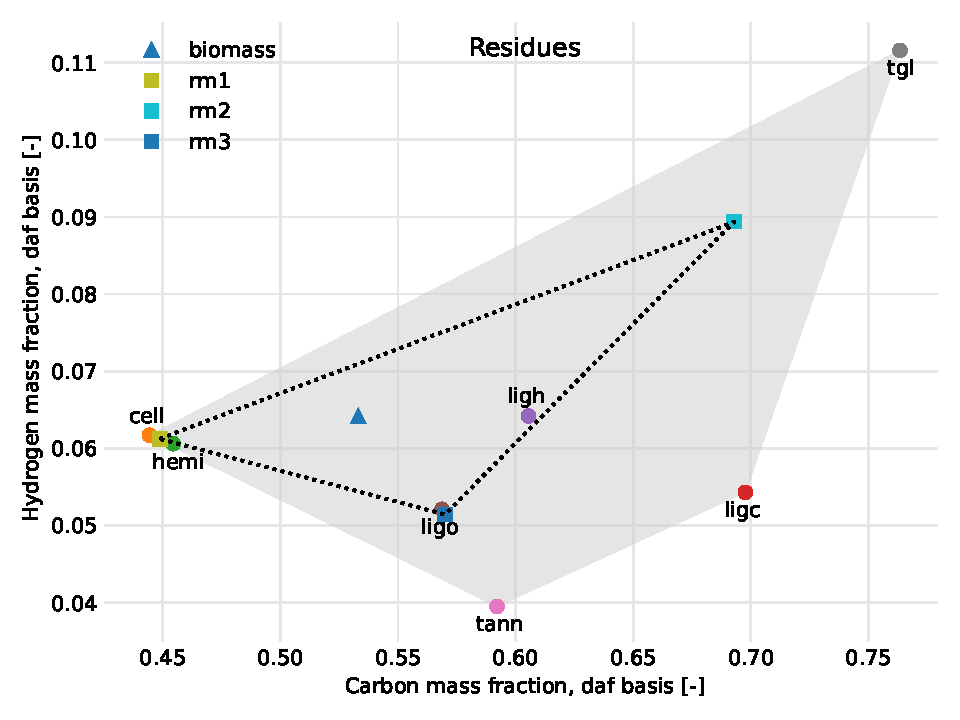
\includegraphics[width=0.8\textwidth]{figures/biocomp-diagram.pdf}
    \caption{Characterization of the Residues feedstock using ultimate analysis data, chemical analysis data, and optimized splitting parameters.}
    \label{fig:biocomp-diagram}
\end{figure}

\subsection{Batch reactor model}

To understand the time-scale and conversion profiles associated with the Debiagi biomass pyrolysis kinetics, the batch reactor model was implemented with the Residues feedstock. Reaction time in the batch model was set to 20 s, a constant reaction temperature of 773.15 K, and a pressure of 101,325 Pa. Figure \ref{fig:batch-biocomp} displays the conversion of the initial biomass concentration with respect to time. All biomass fractions are converted to products within 10 s except for the tannins. All pyrolysis products appear to be generated within 10 s of reaction time as demonstrated by Figure \ref{fig:batch-products}. Final mixture yields are approximately 15 wt. \% gas, 57 wt. \% liquids, 13 wt. \% solids, and 14 wt. \% metaplastics which suggests a total solids yield of 27 wt. \%.

\begin{figure}[H]
    \centering
    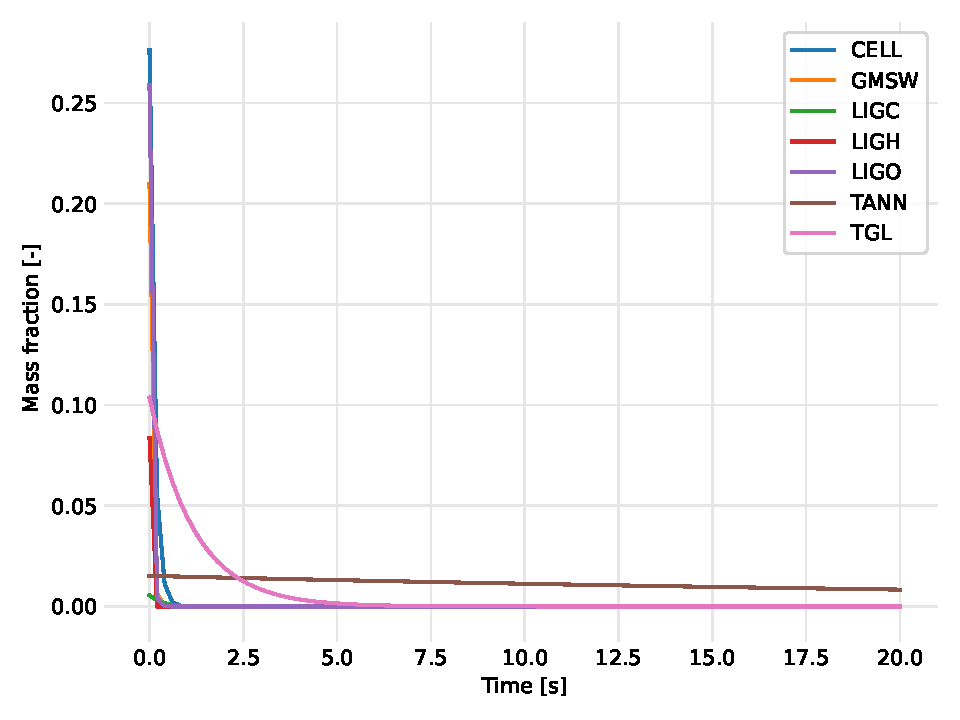
\includegraphics[width=0.8\textwidth]{figures/batch-biocomp.pdf}
    \caption{Conversion profiles of the biomass composition for the Residues feedstock.}
    \label{fig:batch-biocomp}
\end{figure}

\begin{figure}[H]
    \centering
    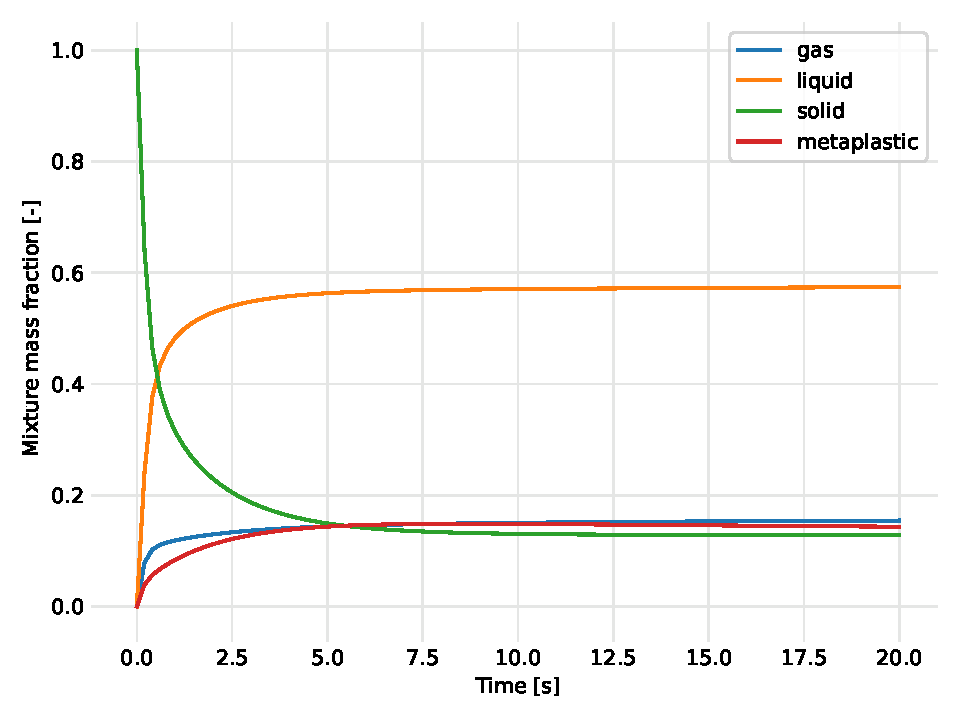
\includegraphics[width=0.8\textwidth]{figures/batch-products.pdf}
    \caption{Generation of the pyrolysis products for the Residues feedstock.}
    \label{fig:batch-products}
\end{figure}

According to the experimental data from the NREL 2FBR, the char yield for the Residues feedstock is around 15 wt. \% compared to the batch reactor model's 27 wt. \% total solids yield. A majority of the solids yield from the batch reactor model is due to the metaplastic species. To increase the metaplastic reaction rates, temperature $T$ was added to the prefactors. For example, the original prefactor for reaction 23 in Table \ref{tab:chem-kinetics} is $5 \times 10^{12}$ while the modified prefactor is $5 \times T \times 10^{12}$. The effects of this modification can be seen in Figure \ref{fig:metaplastic} where the metaplastic yield for the Residues feedstock is considerably less than the yield from the original reaction rates. Total solids yield using the modified reaction rates is approximately 18 wt. \% compared to 27 wt. \% using the original reaction rates. The remaining reactor models presented in this report use the modified metaplastic reaction rates since the total solids yield more closely resembles the NREL 2FBR char yield.

\begin{figure}[H]
    \centering
    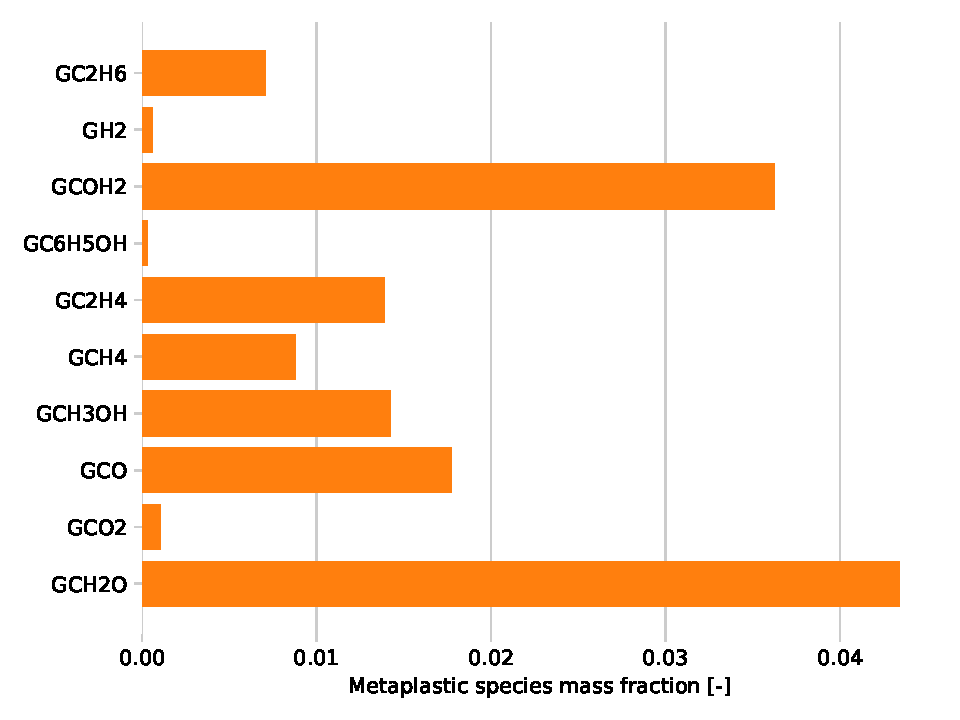
\includegraphics[width=0.49\textwidth]{figures/metaplastic1.pdf}
    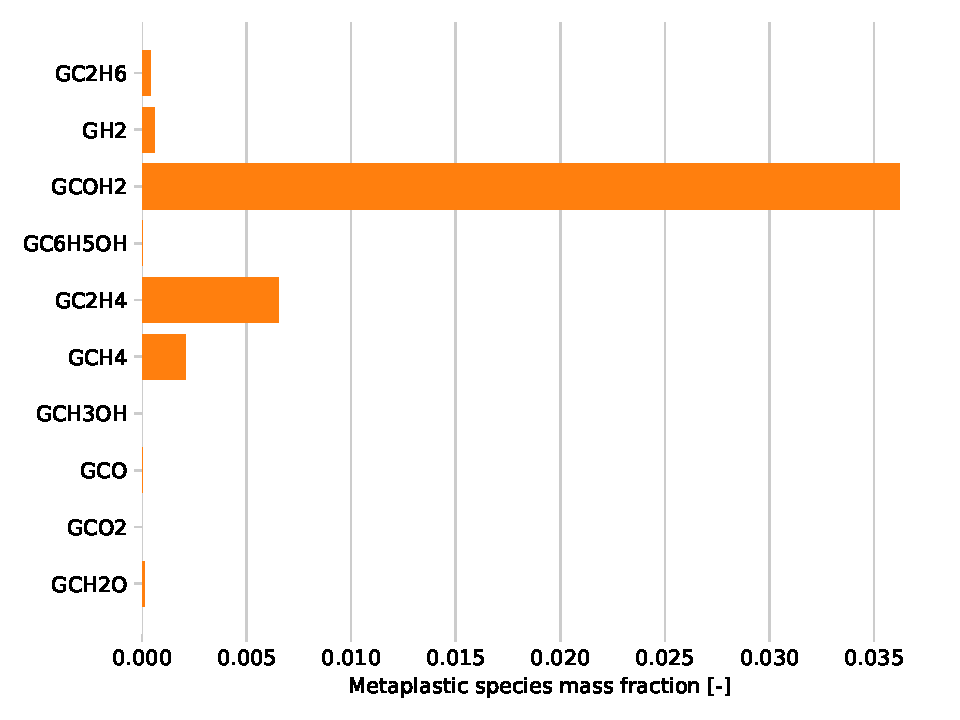
\includegraphics[width=0.49\textwidth]{figures/metaplastic2.pdf}
    \caption{Metaplastic yields for the Residues feedstock using the original (left) and modified (right) reaction rates in a batch reactor model.}
    \label{fig:metaplastic}
\end{figure}

\subsection{CSTR model}

Here.
